\documentclass[12pt,a4paper,oneside]{article}

\usepackage[utf8]{inputenc}
\usepackage[portuguese]{babel}
\usepackage[T1]{fontenc}
\usepackage{amsmath}
\usepackage{amsfonts}
\usepackage{amssymb}
\usepackage{graphicx}
\usepackage{xcolor}
% Definindo novas cores
\definecolor{verde}{rgb}{0.25,0.5,0.35}

\author{\\Universidade Federal de Goiás (UFG) - Câmpus Jataí\\Bacharelado em Ciência da Computação \\Teoria da Computação \\Esdras Lins Bispo Jr.}

\date{14 de abril de 2014}

\title{\sc \huge Primeiro Teste}

\begin{document}

\maketitle

{\bf ORIENTAÇÕES PARA A RESOLUÇÃO}

\begin{itemize}
	\item A avaliação é individual, sem consulta;
	\item A pontuação máxima desta avaliação é 10,0 (dez) pontos, sendo uma das 06 (seis) componentes que formarão a média final da disciplina: quatro testes, uma prova e exercícios;
	\item A média final ($MF$) será calculada assim como se segue
	\begin{eqnarray}
		MF & = & MIN(10, S) \nonumber \\
		S & = & (\sum_{i=1}^{4} 0,2.T_i ) + 0,2.P  + 0,1.E \nonumber
	\end{eqnarray}
	em que 
	\begin{itemize}
		\item $S$ é o somatório da pontuação de todas as avaliações,
		\item $T_i$ é a pontuação obtida no teste $i$,
		\item $P$ é a pontuação obtida na prova, e
		\item $E$ é a pontuação total dos exercícios.
	\end{itemize}
	\item O conteúdo exigido desta avaliação compreende o seguinte ponto apresentado no Plano de Ensino da disciplina: (1) Teoria da Computação.
\end{itemize}

\begin{center}
	\fbox{\large Nome: \hspace{10cm}}
	\fbox{\large Assinatura: \hspace{9cm}}
\end{center}

\newpage

\begin{enumerate}

	\item (5,0 pt) Dado o AFN $M$ abaixo
	\begin{center}
  		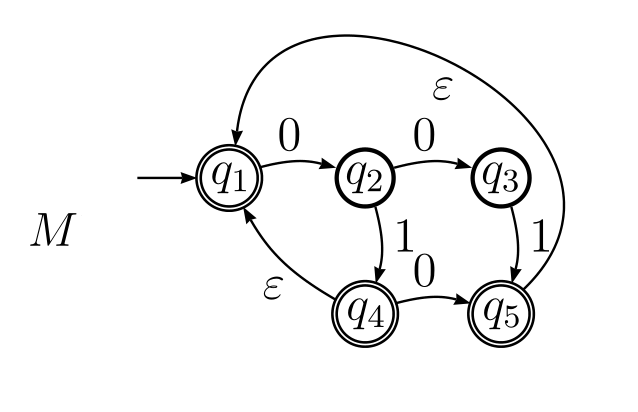
\includegraphics[height=.2\textheight]{imagens/afn.png}
	\end{center}
		
	mostre que:			 
	\begin{enumerate}
		\item (2,5 pt) {\tt 0101} $\in L(M)$ \\
		{\color{verde}
		{\tt 0101} $\in L(M)$ se $M$ aceita {\tt 0101}. Logo existe uma sequência de estados de $M$ que satisfaz a definição formal de computação para um AFN. Seja a sequência de estados $(q_1, q_2, q_4, q_1, q_2, q_4)$. Garantimos que: (i) $q_1$ é o estado inicial; (ii) a sucessão dos estados é válida, pois:
		\begin{itemize}
			\item $q_2 \in \delta(q_1,0)$;
			\item $q_4 \in \delta(q_2,1)$;
			\item $q_1 \in \delta(q_4,\epsilon)$;
			\item $q_2 \in \delta(q_1,0)$;
			\item $q_4 \in \delta(q_2,1)$;
		\end{itemize}
		e (iii) $q_4$ é um estado final. Então $M$ aceita {\tt 0101} e {\tt 0101} $\in L(M)$. $\blacksquare$
		}
		\item (2,5 pt) {\tt 00100} $\not\in L(M)$ \\
		{\color{verde}
		{\tt 00100} $\not\in L(M)$ se $M$ rejeita {\tt 00100}. Logo nenhuma sequência de estados de $M$ satisfaz a definição formal de computação para um AFN. Ao ler a cadeia de entrada {\tt 00100}, $M$ gera apenas dois ramos de computação: (a) um gera a sequência de estados $(q_1, q_2, q_3, q_5, \emptyset, \emptyset)$; e (b) o outro gera a sequência $(q_1, q_2, q_3, q_5, q_1,$ $q_2, q_3)$. Tanto a sequência (a) quanto a sequência (b) não são computações válidas, pois $\emptyset$ e $q_3$ não são estados de aceitação de $M$, respectivamente. Então $M$ rejeita {\tt 00100} e {\tt 00100} $\not\in L(M)$. $\blacksquare$
		}
	\end{enumerate}
	
	\newpage
	\item (5,0 pt) Mostre que a classe das linguagens regulares é fechada sob a operação de complemento.\\
	{\color{verde}
	{\bf Prova:} Seja $A$ uma linguagem regular. A classe de linguagens regulares é fechada sob a operação de complemento se $\overline{A}$ for regular. $\overline{A}$ é regular se for possível construir um AFD $M$ que a reconheça (Definição 1.16).

Seja $M_A = ( Q_A, \Sigma, \delta_A, q_A, F_A )$ o AFD que reconhece a linguagem $A$ (Definição 1.16). Iremos construir o AFD $M = ( Q, \Sigma, \delta, q_0, F )$ a partir de $M_A$. $M$ pode ser construído como se segue:

\begin{enumerate}
	\item $Q = Q_A$;
	\item $\Sigma$ (o mesmo alfabeto para ambas as máquinas);
	\item $\delta = \delta_A$;
	\item $q_0 = q_A$;
	\item $F = \overline{F_A}$.
\end{enumerate}

Como é possível construir $M$, então $\overline{A}$ é regular. Logo, a classe de linguagens regulares é fechada sob a operação de complemento. $\blacksquare$
	}
	
\end{enumerate}

\end{document}